\documentclass[12pt]{beamer}

\mode<presentation>
{
  \usetheme{Madrid}

  \setbeamercovered{transparent=15}
}

\usepackage{graphicx}

\usepackage[clock]{ifsym}

\usepackage[font=Times,timeinterval=29, timeduration=80, timedeath=0, fillcolorwarningsecond=white!60!yellow,
timewarningfirst=50,timewarningsecond=80]{tdclock}

\usepackage[brazil]{babel}

\usepackage[utf8]{inputenc}

\usepackage{times}
\usepackage[T1]{fontenc}

\usepackage{color}

\usepackage{listings}

\lstnewenvironment{scalalang}{%
\lstset{frame=single,escapeinside=`',
  backgroundcolor=\color{yellow!20},
  basicstyle=\footnotesize \ttfamily}
}{}

\lstnewenvironment{javalang}{%
\lstset{frame=single,escapeinside=`',
  backgroundcolor=\color{orange!20},
  basicstyle=\footnotesize \ttfamily}
}{}

\newenvironment{scala}{
\begin{block}{Scala} \begin{semiverbatim}
}{
\end{semiverbatim} \end{block}
}

\newenvironment{java}{
\protect\begin{block}{Java}
\protect\begin{semiverbatim}
}{
\protect\end{semiverbatim}
\protect\end{block}
}

\title{Introdução à Programação em Scala}
\author[João Rafael]{João Rafael Moraes Nicola}
\institute[PPGI-DI-UFES]
{
        Programa de Pós-Graduação em Informática\\
        Departamento de Informática\\
        Universidade Federal do Espírito Santo
}

\date[DWWS]{\today}


\subject{Scala}



% If you have a file called "university-logo-filename.xxx", where xxx
% is a graphic format that can be processed by latex or pdflatex,
% resp., then you can add a logo as follows:

\pgfdeclareimage[height=1cm]{university-logo}{UFES_1_COR_0.png}
\logo{\pgfuseimage{university-logo}}



% Delete this, if you do not want the table of contents to pop up at
% the beginning of each subsection:
\AtBeginSubsection[]
{
  \begin{frame}<beamer>{Índice}
    \tableofcontents[currentsection,currentsubsection]
  \end{frame}
}


%\beamerdefaultoverlayspecification{<+->}


\begin{document}

\begin{frame}

\initclock

\titlepage

\end{frame}
  
\date{\cronominutes ~ ~ \resetcrono{\raisebox{-0.5ex}{\StopWatchStart}}}


\begin{frame}{Indice}
  \tableofcontents
\end{frame}


\section{Outra linguagem ?!} 

\begin{frame}{Para quê aprender uma outra linguagem?}

\begin{itemize}
        \item Todas as linguagens de uso geral são igualmente expressivas (Máquina de Turing)
        \pause
        \item O mercado de TI no Brasil exige primariamente conhecimento em Java.
        \pause
        \item A linguagem de programação em si não é importante. O importante é o processo de desenvolvimento, 
              qualidade das ferramentas, bibliotecas, etc.
        \pause
        \item Já me formei, não quero estudar mais.
\end{itemize}

\end{frame}

\begin{frame}{Para quê aprender uma outra linguagem?}

\begin{block}{Expressividade}
 Todas as linguagens de uso geral são igualmente expressivas
\end{block}
\pause
\begin{enumerate}
\item Se distinguem sintaticamente 
\pause
\item Se distinguem pragmáticamente
\end{enumerate}
\end{frame}

\begin{frame}{Para quê aprender uma outra linguagem?}
\begin{block}{Mercado}
O mercado de TI no Brasil exige primariamente conhecimento em Java.
\end{block}
\pause
\begin{enumerate}
        \item O mercado muda e os paradigmas também.
        \pause
        \item A 3 anos atrás, Cobol era (ou é ainda) a linguagem mais 
              usada nos ambientes corporativos.
        \pause
        \item Vamos cometer o mesmo erro de nossos pais (na profissão)?
\end{enumerate}
\end{frame}

\begin{frame}{Para quê aprender uma outra linguagem?}
\begin{block}{Processo}
        A linguagem de programação em si não é importante. 
        O importante é o processo de desenvolvimento, 
              qualidade das ferramentas, bibliotecas, etc.
\end{block}
\pause
\begin{alertblock}{}
Deve ser por isso que todo mundo ainda programa em FORTRAN e Assembler!
\end{alertblock}
\end{frame}

\begin{frame}{Para quê aprender uma outra linguagem?}
\begin{block}{Preguiça}
        Já me formei, não quero estudar mais.
\end{block}
\pause
\begin{alertblock}{}
        Essa desculpa vocês não têm!
\end{alertblock}
\end{frame}

\begin{frame}{Para quê aprender uma outra linguagem?}
\begin{quote}
``As linguagens que falamos afetam nossas percepções sobre mundo'' (Lera Boroditsky, 2011)

\bigskip

``É tentador, se a única ferramenta que você tiver for um martelo, tratar tudo como se fosse um prego.'' (Abraham Maslow, 1966)

\bigskip

\url{http://hammerprinciple.com/therighttool}

\end{quote}
\end{frame}

\section{Scala}

\subsection{De Java para Scala}

\begin{frame}[fragile]{Hello World!}

 \begin{java}
class HelloWorld \{
  public static void main(String[] args) \{
    System.out.println("Hello World!")
  \}
\}
 \end{java}
 
 \pause
 
 \begin{scala}
object HelloWorld extends App \{
    println("Hello World!")
\}
 \end{scala}

\end{frame}

\begin{frame}[fragile]{Classes}

\begin{java}
package x.y.z;

public class A extends B implements C, D {
}
\end{java}
\pause
\begin{scala}
package x.y.z

class A extends B with C with D
\end{scala}

\end{frame}

\begin{frame}[fragile]{Interfaces}

\begin{java}
public interface A extends B, C {
}
\end{java}
\pause
\begin{scala}
trait A extends B with C 
\end{scala}

\end{frame}

\begin{frame}[fragile]{Atribuição}
\begin{java}
Map<String,Integer> m = 
   new HashMap<String,Integer>();
\vdots final int xyz = 12;
\end{java}
\pause
\begin{scala}
var m = new HashMap[String,Integer]()
\vdots val xyz = 12
\end{scala}
\end{frame}

\begin{frame}[fragile]{Sigletons}

\begin{onlyenv}<1>
\begin{java}
public class T \{
  private static T instance = null;
  public static T getInstance() \{
    synchronized(this) \{
      if(instance == null) \{
        instance = new T();
      \}
      return instance;
     \}
  \}
\}
\dots
T obj = T.getInstance();
obj.method();
\end{java}
\end{onlyenv}

\begin{onlyenv}<2>
\begin{scala}
object T
\dots
T.method()
\end{scala}
\end{onlyenv}

\end{frame}

\begin{frame}[fragile]{Métodos}
\begin{java}
\small
class C \{
  public String metodo(int x, double y, Obj o) \{
    \dots
  \}
\}
\end{java}
\pause
\begin{scala}
\footnotesize
class C \{
  def metodo(x : Int, y : Double, o : Obj) : String = \{
    \dots
  \}
\}  
\end{scala}
\end{frame}

\begin{frame}[fragile]{Classes de Domínio}
\begin{columns}[t]
\begin{column}{5cm}

\tiny
\begin{java}
class Retangulo implements Serializable, 
   Comparable<Retangulo> \{
  private final double width;
  private final double height;
  public Retangulo(double width, 
                   double height) \{
    this.width = width;
    this.height = height;
  \}
  public Double getWidth() \{
    return width;
  \}
  public Double getHeight() \{
    return height;
  \}
  public String toString() \{
    return "Retangulo(" + width + 
    "," + height + ")";
  \}
  public boolean equals(Object O) \{
    \dots
  \}
\end{java}  
\end{column}

\begin{column}{5cm}
\tiny
\begin{block}{}

\begin{semiverbatim}
  public int compareTo(Retangulo r) \{ 
    \dots
  \}
  public int hashCode() \{
    \dots
  \}
\}
\end{semiverbatim}
\end{block}

\pause

\begin{scala}
case class Retangulo(
  width : Double, height : Double)
\end{scala}
\end{column}
\end{columns}
\end{frame}


\subsection{Scala além do Java} % 10 min (27 min)

\begin{frame}[fragile]{Inferência de tipos}
\begin{scala}
val x = "aaaaaa" // x : String

val y = 12 +  x.length // y : Int

val m = Array("abc", "de", "f") 
// m : Array[String]

val z = m map (_.length) // z : Array[Int]
\dots
\end{scala}
\end{frame}

\begin{frame}[fragile]{Tuplas}
\begin{scala}
def toPolar(x : Double, y : Double) = 
  (math.sqrt(x*x+y*y), math.atan(x,y))
// toPolar :: (Double,Double) => (Double,Double)

val (mag,ang) = toPolar(3,4)
// mag : Double, ang : Double
\end{scala}
\end{frame}

\begin{frame}[fragile]{Aplicação parcial (currying)}
\scriptsize
\begin{scala}
def quicksort[T](
      le_pred : (T,T) => Boolean)(
      data : Vector[T]) : Vector[T] =
  if(data.length <= 1) 
   \{ data \} else \{
      val pivot = data.head
      val (le,g) = 
        data.tail.partition(le_pred)
      quicksort(le_pred)(le) ++ 
        Vector(pivot) ++ 
        quicksort(g)
  \}

//quicksort para strings
val quicksortString = 
  quicksort[String](_ <= _)

//quicksort para ints (decrescente)
val quicksortInt = 
  quicksort[Int](_ >= _)
\end{scala}
\end{frame}

\begin{frame}[fragile]{Traits}
Múltipla herança (\emph{mixins}):
\begin{columns}[t]
\scriptsize
\column{5.5cm}
\begin{scala}
trait A \{
  def metodo1(x : Int) =
    x + metodo2(x)
  def metodo2(x : Int) : Int
\}

trait B \{
  def metodo2(x : Int) = 
    x * metodo3(x)
  def metodo3(x : Int) : Int
\}

trait C \{
  def metodo2(x : Int) = x * 5
\}
\end{scala}

\column{6cm}
\begin{block}{}
\begin{semiverbatim}
class D extends A with B \{
  def metodo3(x : Int) = x - 2
\}

println(new D().metodo1(10)) 
//imprime: 90

println((new A with C).metodo1(10)) 
//imprime: 60
\end{semiverbatim}
\end{block}
\end{columns}
\end{frame}

\begin{frame}[fragile]{Direitos iguais}
\begin{itemize}
\item Em Scala, todos os tipos herdam de \texttt{scala.Any}
\pause
\item Não há distinção entre \emph{Boxed} e \emph{Unboxed} types.
\end{itemize}
\pause
\begin{scala}
(1 to 10) foreach println
//imprimes os números de 1 a 10
\end{scala}
\end{frame}

\begin{frame}[fragile]{Casamento de padrões}
\scriptsize
\begin{scala}
abstract sealed class Expr
case class Val(n : Int) extends Expr
case class Plus(e1 : Expr, e2 : Expr) extends Expr
case class Minus(e1 : Expr, e2 : Expr) extends Expr
case class Times(e1 : Expr, e2 : Expr) extends Expr
case class Div(e1 : Expr, e2 : Expr) extends Expr

def eval(e : Expr) : Int = e match \{
  case Val(n) => n
  case Plus(e1,e2) => eval(e1) + eval(e2)
  case Minus(e1,e2) => eval(e1) - eval(e2)
  case Times(e1,e2) => eval(e1) * eval(e2)
  case Div(e1,e2) => eval(e1) / eval(e2)
\}

println(eval(
  Times(Val(5),Plus(Val(2),Val(3)))))
//Imprime: 25
\end{scala}
\end{frame}

\begin{frame}[fragile]{Expressões lambda}
\footnotesize
\begin{scala}
val f1 = (x : Int, y : Int) => x + y
//f1 : (Int,Int) => Int
val f2 : (Int,Int) => Int = (_ + _)
//f2 = f1
val f3 : List[Int] => Int = \{
   case List() => 0
   case List(x) => x
   case List(x,y) => x * y
   case l => l.sum
\}
val f5 = (x : Int) => x * 10
val f6 = f3 andThen f5

println(f6(List(1,2,3,4,5)))
//imprime: 150

\end{scala}
\end{frame}

\begin{frame}[fragile]{Call-by-name}
\scriptsize
\begin{scala}
class Logger \{
  var level : Int = 2
  def info(msg : => String) =
    if (level > 3) \{ println(msg) \} else \{ \}
\}

def costlyOp() = \{
  Thread.sleep(5000)
  "done"
\}

val logger = new Logger
logger.info(costlyOp())
//Não imprime nada nem executa 
//a expressão do parâmetro

logger.level = 4
logger.info(costlyOp())
//Agora espera 5 segs e imprime "done"
\end{scala}
\end{frame}

\begin{frame}[fragile]{Expressões Regulares}
\footnotesize
\begin{scala}
val re1 = """(\\d\\d\\d\\d)-(\\d\\d)-(\\d\\d)"""r
val re2 = """(\\d\\d)/(\\d\\d)/(\\d\\d\\d\\d)"""r

def parseDate(t : String) = t match \{
  case re1(ano,mes,dia) => (ano,mes,dia)
  case re2(dia,mes,ano) => (ano,mes,dia)
  case _ => 
    throw new RuntimeException(
        s"Invalid date: \$\{t\}")
\}

println(parseDate("2009-12-02"))
println(parseDate("02/12/2009"))
\end{scala}
\end{frame}

\begin{frame}{Outras Características}

\emph{Parser combinators}, \emph{Actors}, \emph{Monads},
diversos tipos de DSLs embutidas (DB, ...),
macros \emph{higiênicas},
interpolação de strings,
API moderna de coleções,
generalização do comando \emph{for},
recursão de cauda,
co/contra-variância,
parâmetros implícitos,
conversões implícitas,
\emph{algebraic data types},
compilação para .NET e para Javascript,
interpretador REPL (\emph{Read-Evaluate-Print Loop}),
\emph{path-dependent types},
sinônimos de tipos,
granularidade fina de controle aos membros da classe
\dots
\end{frame}

\subsection{Coleções} % 10 min (55 min)

\begin{frame}[fragile]{Coleções}
\scriptsize
\begin{columns}[t]
\column{5.5cm}
\begin{scala}
val x = (0 until 100).to[Vector] 
val y = x map (_ + 5) 
          filter (_ < 10)
val z1 = (2 to 5) flatMap 
          (t => x map (t * _))
val z2 = for \{ 
            a <- 0 until 100
            b = a + 5
            if b < 10
            t <- 2 to 5
          \} yield (t * a)

def costlyOp(x : Int) = \{
  Thread.sleep(
   (math.random * 100.0).toLong)
  x * 5
\}
\end{scala}
\column{5.5cm}
\begin{block}{}
\begin{semiverbatim}
def chrono[T](op : => T) = \{
  val s = System.nanoTime
  val res = op
  val e = 
    (System.nanoTime-s)
     .toDouble / 1e9
  println(
     s"elapsed: $\{elapsed\} s")
  (elapsed,res)
\}

val (st,_) = chrono \{
  x map (costlyOp) 
    foreach(_ => ())
\}
val (pt,_) = chrono \{
  x.par map (costlyOp) 
    foreach(_ => ()))
\}
println(
  s"speedup: $\{seqTime/parTime\}")
\end{semiverbatim}
\end{block}
\end{columns}
\end{frame}

\begin{frame}[fragile]{Coleções}
\begin{scala}
val m = Map(1 -> "Joao", 2 -> "Pedro", 
            3 -> "Andre")
val m1 = m map \{ case (x,y) => (y,x) \}
println(s"m1 = $\{m1\}")
val s = (2 to 10).collect(m).to[Set]
val s2 = s -- Set("Pedro")
println(s"s2 = $\{s2\}")
val m3 = (1 to 100).groupBy(_ \% 5)
println("m3:")
m3 foreach \{ 
  case (k,l) => 
   println(s"   $k: $\{l.mkString(",")\}") 
\}
\end{scala}
\end{frame}

\begin{frame}[fragile]{Coleções}
\scriptsize
\begin{scala}
import java.io._
import scala.io.Source

val pw = new PrintWriter(
    new FileWriter("test.csv"))
List(1 to 5, 6 to 10, 11 to 15).
  foreach(l => pw.println(l.mkString("\\t")))
pw.close()

val res = (
  Source.fromFile(new File("test.csv"))
    .getLines
    .map(_.split("\\\\t").filter(_.trim != ""))
    .collect \{ 
       case Array(x1,_,_,_,x2) => 
         (x1.toDouble,x2.toDouble) 
     \}
    .map \{ case (x1,x2) => x1 * x2 \}
    .reduce(_ + _)
  )
println(res)    

\end{scala}
\end{frame}

\section{APIs Scala}
\begin{frame}{APIs}
\begin{itemize}
\item Programs Scala tem acesso à todas APIs disponíveis na JVM
\pause
\item Frequentemente é mais fácil usar as APIs pelo Scala
\pause 
\item Existe uma grande quantidade de APIs para o Scala que
\begin{enumerate}
  \item fazem uso dos recursos do Scala para construir DSLs
  \pause
  \item exploram o sistema de tipos do Scala
  \pause
  \item encaixam-se melhor no paradigma funcional
\end{enumerate}
\end{itemize}
\end{frame}

\begin{frame}{Frameworks Web}
\begin{itemize}
\item Play! Framework
\item Lift
\item Scalatra
\item Spray
\item \dots
\end{itemize}
\end{frame}

\begin{frame}{Persistence}
\begin{itemize}
\item Slick
\item Sorm
\item Squeryl
\item Scala ActiveRecord
\item \dots 
\end{itemize}
\end{frame}

\begin{frame}{Testing}
\begin{itemize}
\item ScalaCheck
\item ScalaTest 
\item Specs2 — Software Specifications for Scala.
\item Scalastyle
\item ScalaMock – Scala native mocking framework
\item \dots
\end{itemize}
\end{frame}

\begin{frame}{Distributed Systems}
\begin{itemize}
\item Akka
\item Finagle 
\item \dots
\end{itemize}
\end{frame}

\begin{frame}{Distributed Systems}
\begin{itemize}
\item Akka
\item Finagle 
\item \dots
\end{itemize}
\end{frame}

\section{Paradigma Funcional $\times$ Paradigma Imperativo} 

\begin{frame}{Lei de Moore}

\begin{quote}
``O número de transístores dos chips dobra à cada 18 meses mantendo o mesmo custo'' (Gordon Moore, 1965)
\end{quote}

\pause

\begin{center}
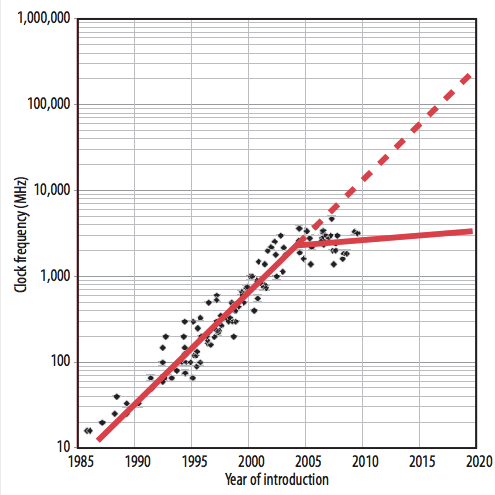
\includegraphics[height=6cm]{cpu_speed.png}
\end{center}

\end{frame}

\begin{frame}{Paralelismo}
\begin{itemize}
\item Processadores \emph{Multi-core}
\pause
\begin{enumerate}
        \item Frequentes em celulares e tablets
        \item Lançamento de 2014: Intel Core i7-5960x,
              com 8 núcleos.
        \item Xeons com 18 núcleos
        \item SPARCs: 128 threads paralelas
\end{enumerate}
\pause
\item Limitação na velocidade por núcleo.
\end{itemize}
\pause
Solução: paralelizar o código!
\end{frame}

\begin{frame}{Paralelismo - Dificuldades}
\begin{itemize}
\item Condições de concorrência
\pause
\begin{enumerate}
\item Deadlocks, livelocks, etc.
\pause
\item Sincronização
\pause
\item Não-determinismo
\pause
\item Caos!
\end{enumerate}
\pause
\item Melhores práticas:
\pause
\begin{enumerate}
\item Evitar contenção
\pause
\item Evitar mudança de estado!
\pause
\item Evitar bloqueios
\pause
\item Usar arquiteturas assíncronas
\pause
\item Evitar mudança de estado!
\pause
\item {\Huge \color{red} Evitar mudança de estado!}
\end{enumerate}
\end{itemize}
\end{frame}

\begin{frame}{Paralelismo}
\begin{itemize}
\item Programação orientada à objeto: ênfase em estados 
\pause
\item Programação funcional: incentiva o desenvolvimento 
      de código independente de mudançã de estados
\pause      
\item Scala: o melhor dos dois mundos!      
\end{itemize}
\end{frame}

\begin{frame}{Fim}
\end{frame}

\end{document}



